\documentclass[]{report}

\usepackage{amsmath,amsfonts}
\usepackage{graphicx}
\usepackage{url}
\usepackage[hidelinks]{hyperref}

% Title Page


\title{{\huge  TITLE} \\
{\small Automatic Control\\
Electronic Engineering for Intelligent Vehicles\\
University of Bologna\\
A.A. 202X-202X}}
\author{Student A and Student B and ...}


\begin{document}
\maketitle

\begin{abstract}
	Here briefly detail  the aims of the project.
\end{abstract}


\documentclass[]{report}
\usepackage{amsmath,amsfonts}
\usepackage{graphicx}
\usepackage{url}
\usepackage[hidelinks]{hyperref}
\usepackage{tikz}
\usetikzlibrary{arrows.meta, decorations.pathreplacing, decorations.pathmorphing}

% Title Page
\title{{\huge  TITLE} \\
{\small Automatic Control\\
Electronic Engineering for Intelligent Vehicles\\
University of Bologna\\
A.A. 202X-202X}}
\author{Student A and Student B and ...}


\begin{document}
\maketitle

\begin{abstract}
	Here briefly detail  the aims of the project.
\end{abstract}

\chapter{Introduction}
\section{Motivations}
Explain why the selected application is important. Describe the application with informal words.

\section{Contributions}
Describe what this project deals with. What has been done to solve the problem presented in the motivations.

\section{State of art and literature comparison}
List the closest works that deal with the same problem and compare the achievement obtained and the strategies exploited in this paper. For the search of the literature use \url{https://ieeexplore.ieee.org/Xplore/home.jsp} and \url{https://www.sciencedirect.com/}.

\section{Organisation of the manuscript}
Describe what the reader finds in each of the Sections of this manuscript.

\section{List of the symbols}
Here list all the symbols used in the manuscript and add a description to each of them (Use the International System of Units \url{https://en.wikipedia.org/wiki/International_System_of_Units}).

\chapter{MAIN BODY}
Change the title with the name of the selected application

\section{Model and Problem Formulation}
In this section, we formulate the control problem for the active suspension system of a half-car model. This system aims to regulate both the vertical position and the perceived pitch angle of the vehicle body, enhancing ride comfort and handling. The model is described by a nonlinear dynamic system influenced by road disturbances, actuator forces, and sensor measurements.

The general form of the system is expressed as:
\begin{align}
	\dot{x} &= f(x, u, w) \\
	y &= h(x, u, w) \\
	e &= h_e(x, u, w)
\end{align}

Where:
\begin{itemize}
	\item $x \in \mathbb{R}^n$ is the \textbf{state vector},
	\item $u \in \mathbb{R}^p$ is the \textbf{control input vector},
	\item $y \in \mathbb{R}^q$ is the \textbf{measured output vector},
	\item $e \in \mathbb{R}^{l_m}$ is the \textbf{control error (goal)},
	\item $d \in \mathbb{R}^{l_d}$ is the \textbf{disturbance vector},
	\item $r \in \mathbb{R}^{l_r}$ is the \textbf{reference signal},
	\item $\nu \in \mathbb{R}^q$ is the \textbf{sensor noise},
	\item $w = \text{col}(d, \nu, r)$ is the \textbf{exogenous input}.
\end{itemize}
\begin{equation}
	\label{eq:FormulaA}
	\begin{aligned}
		\dot{x} &= f(x,u) && x(t_0) = x_0
\\
y &= h(x,u)
\end{aligned}
\end{equation}
\subsection*{Assumptions}

To make the problem tractable and to ensure solvability of the control task, we impose the following assumptions:

\begin{enumerate}
	\item The exogenous input $w$ is not directly measurable.
	\item Disturbances $d$ are bounded.
	\item Reference signal $r$ and its first derivatives are known.
	\item Bounded disturbances imply bounded internal states and outputs.
	\item The system has at least as many control inputs as control goals, i.e., $p \geq l_m$.
	\item The control error $e$ can be reconstructed from the output $y$: $\exists E$ such that $e = E(y)$.
\end{enumerate}

These assumptions lay the theoretical foundation required to design a control law capable of driving the error $e$ to zero despite the presence of unknown disturbances and sensor noise.

\section{Model Analysis}
\subsection{Dynamic Model}

The dynamic behavior of the half-car is described using a state vector that captures both translational and rotational aspects of motion, as well as external road-induced disturbances. The state vector consists of six components and is expressed as follows:
\begin{align}
	x = \begin{bmatrix}
		x_1 \\ x_2 \\ x_3 \\ x_4 \\ x_5 \\ x_6
	\end{bmatrix} =
	\begin{bmatrix}
		z - z_g \\
		\dot{z} - \dot{z}_g \\
		\theta \\
		\dot{\theta} \\
		\theta_g \\
		\omega_g
	\end{bmatrix}
\end{align}

Here, $z$ represents the vertical displacement of the vehicle’s center of mass (CoM), while $z_g$ denotes the vertical road disturbance. The variable $\dot{z}$ is the vertical velocity of the vehicle body, and $\theta$ is the pitch angle, which describes the rotation of the vehicle body about its lateral axis. The pitch rate is given by $\dot{\theta}$. The disturbance inputs include the road pitch angle $\theta_g$ and its time derivative $\omega_g = \dot{\theta}_g$, which captures the rate of change of the road gradient. Therefore, the state vector effectively captures the relative vertical and angular positions and velocities of the vehicle body with respect to the road surface.


\newpage

The suspension system in the half-car model is influenced by two actuators—one at the front and one at the rear. These actuators generate forces that contribute to both the vertical and rotational dynamics of the vehicle body. The control input vector is defined as:


\begin{align}
	u = \begin{bmatrix}
		u_1 \\
		u_2
	\end{bmatrix} =
	\begin{bmatrix}
		f_{af} + f_{ar} \\
		f_{af} d_f - f_{ar} d_r
	\end{bmatrix}
\end{align}

In this expression, $f_{af}$ and $f_{ar}$ are the forces generated by the front and rear suspension actuators, respectively. The parameters $d_f$ and $d_r$ denote the distances from the vehicle's center of mass to the front and rear axles. The first control input, $u_1$, represents the total vertical force acting on the vehicle body due to both actuators. The second input, $u_2$, represents the net moment about the vehicle’s center of mass generated by these forces, which directly influences the pitch motion.


The evolution of the system over time is governed by a set of first-order differential equations derived from Newton’s second law for translational and rotational motion. The dynamic model is written as:


\begin{align}
	\dot{x} = \begin{bmatrix}
		x_2 \\
		f_2 - \ddot{z}_g \\
		x_4 \\
		f_4 \\
		x_6 \\
		\alpha_g
	\end{bmatrix}
\end{align}

In this representation, $f_2$ is the vertical acceleration of the vehicle body, given by:

\begin{align}
	f_2 &= -g + \frac{1}{m}(f_{sf} + f_{sr}) + \frac{u_1}{m} \\
\end{align}

The pitch angular acceleration $f_4$ is given by:

\begin{align}	
	f_4 &= \frac{1}{J}(f_{sf} d_f - f_{sr} d_r + u_2 + f_{wf} l_{f} + f_{wr} l_{r})
\end{align}


The suspension deflections and velocities are:

\begin{align}
	s_1 &= x_1 + d_f(\sin x_3 - \sin x_5), \quad s_3 = x_1 - d_r(\sin x_3 - \sin x_5) \\
	s_2 &= x_2 + d_f(x_4 \cos x_3 - x_6 \cos x_5), \quad s_4 = x_2 - d_r(x_4 \cos x_3 - x_6 \cos x_5)
\end{align}

Suspension forces are modeled as spring-damper systems:

\begin{align}
	f_s(p, v) = -k p - \beta v
\end{align}

\subsection{Sensor Model}

The vehicle is equipped with a set of onboard sensors that provide real-time measurements required for control and state estimation. These sensors include two accelerometers, a gyroscope, and two suspension potentiometers. The complete sensor output is gathered in the measurement vector:

\begin{align}
	y = \begin{bmatrix}
		y_y \\ y_z \\ y_g \\ y_l \\ y_r
	\end{bmatrix} =
	\begin{bmatrix}
		\sin x_3(f_2 + g) + \cos x_3(f_{wr} + f_{wf})/m \\
		\cos x_3(f_2 + g) - \sin x_3(f_{wr} + f_{wf})/m \\
		x_4 \\
		s_1 \\
		s_3
	\end{bmatrix} + \nu
\end{align}

\paragraph{Accelerometers.}
The first two components of the vector, $y_y$ and $y_z$, correspond to the lateral and vertical accelerations measured in the vehicle's body-fixed frame. These quantities are nonlinear combinations of the vertical acceleration of the center of mass and the contributions from external lateral forces, projected into the rotating frame of the vehicle using the pitch angle $x_3 = \theta$. These measurements reflect how the vehicle responds dynamically to road inputs and control actions, and are essential for estimating the apparent pitch felt by passengers.

\paragraph{Gyroscope.}
The third measurement, $y_g$, provides a direct reading of the pitch rate $\dot{\theta}$ (i.e., $x_4$). This is obtained from a gyroscope mounted on the vehicle, and it offers high-frequency dynamic information critical for closed-loop control, especially in active suspension systems that respond rapidly to body motion.

\paragraph{Suspension Potentiometers.}
The last two measurements, $y_l$ and $y_r$, represent the deflections of the left and right suspensions, respectively. These are measured via linear potentiometers or displacement sensors mounted along each suspension strut. The quantities $s_1$ and $s_3$ represent how much each suspension has compressed or extended relative to its rest position. These values reflect road unevenness and the vehicle's dynamic posture (e.g., roll or pitch), and are fundamental for both control and diagnostic purposes.

\paragraph{Sensor Noise.}
All measurements are affected by additive noise $\nu = [\nu_y, \nu_z, \nu_g, \nu_l, \nu_r]^T$, which accounts for sensor imperfections, electrical disturbances, or vibration-induced errors. The presence of noise highlights the importance of robust control and filtering strategies in practical implementations.


\subsection{Control Objectives}

We define the apparent pitch angle $\theta_a$ using accelerometer data:

\begin{align}
	\theta_a = \sin^{-1} \left( \frac{y_y}{\sqrt{y_y^2 + y_z^2}} \right)
\end{align}

The control error vector is defined as:

\begin{align}
	e = \begin{bmatrix}
		\frac{y_f d_r + y_r d_f}{d_r + d_f} - r_z \\
		\theta_a - r_\theta
	\end{bmatrix}
\end{align}

This error describes deviations from the desired vertical height and perceived pitch. The control task is to design $u$ to drive $e \rightarrow 0$ in the presence of disturbances and noise.

The second component of the error vector $he(x,u,w)$ captures the deviation from a desired apparent pitch angle $\theta_a$, which reflects the passenger-perceived acceleration. It is defined through the nonlinear relationship:
\[
\sin(\theta_a) = \frac{y_y}{\sqrt{y_y^2 + y_z^2}} \quad \Rightarrow \quad \theta_a = \sin^{-1}\left(\frac{y_y}{\sqrt{y_y^2 + y_z^2}}\right),
\]
where $y_y$ and $y_z$ are the accelerometer outputs along the body-frame $y$ and $z$ axes, respectively. This formulation provides an estimate of the pitch experienced by passengers during acceleration, braking, or uneven ground contact.


The complete output error function thus becomes:
\[
he(x, u, w) =
\begin{bmatrix}
	\displaystyle \frac{(s_1 + \nu_f) d_r + (s_3 + \nu_r) d_f}{d_r + d_f} - r_z \\
	\displaystyle \sin^{-1}\left( \frac{h_1 + \nu_y}{\sqrt{(h_1 + \nu_y)^2 + (h_2 + \nu_z)^2}} \right) - r_\theta
\end{bmatrix},
\]
where $s_1$, $s_3$ are suspension deflections, $h_1$, $h_2$ are derived from dynamic equations, and $\nu_i$ are sensor noise terms. This formulation ensures the controller minimizes both height and perceptual pitch deviations.

\section{Proposed Solution}
Here describe the proposed solution: Control system architecture (draw a block scheme!), mathematical description of the solution, listings of the MATLAB code implemented to obtain the solution

\subsection{Sensor Model}

The effectiveness of the control architecture relies heavily on the accurate and timely acquisition of physical quantities related to the vehicle's motion and posture. To this end, the half-car system is equipped with a set of onboard sensors, specifically selected to ensure observability of the dynamic model and to allow real-time feedback control.

\paragraph{Measurement Vector.}
The complete sensor output is gathered in the measurement vector:

\begin{align}
	y = \begin{bmatrix}
		y_y \\ y_z \\ y_g \\ y_l \\ y_r
	\end{bmatrix} =
	\begin{bmatrix}
		\sin x_3(f_2 + g) + \cos x_3(f_{wr} + f_{wf})/m \\
		\cos x_3(f_2 + g) - \sin x_3(f_{wr} + f_{wf})/m \\
		x_4 \\
		s_1 \\
		s_3
	\end{bmatrix} + \nu
\end{align}

This vector includes measurements from two accelerometers, one gyroscope, and two linear potentiometers, all subject to additive noise $\nu$.

\paragraph{Accelerometers.}
The first two components $y_y$ and $y_z$ represent the lateral and vertical accelerations measured in the vehicle’s body-fixed reference frame. These measurements are obtained via two MEMS accelerometers mounted at the vehicle's center of mass. Due to the non-inertial frame of reference, the accelerations are nonlinear combinations of translational and rotational dynamics and include the gravitational component projected along the vehicle's pitch angle $x_3 = \theta$.

These measurements are used to estimate the apparent pitch angle $\theta_a$, which is a key feedback signal for pitch stabilization control. We assume a typical sensor such as the \textbf{STMicroelectronics LIS3DH}, offering 12-bit resolution, low noise density ($\sim50~\mu g/\sqrt{Hz}$), and a digital output interface.

\paragraph{Gyroscope.}
The third component $y_g$ corresponds to the pitch angular rate $\dot{\theta}$, measured directly by a gyroscope mounted on the vehicle frame. This measurement provides high-frequency information essential for dynamic feedback control and stability monitoring.

A typical device used could be the \textbf{Bosch BMI160} inertial measurement unit (IMU), with integrated accelerometer and gyroscope, capable of delivering low-latency angular rate data with high sensitivity (16-bit ADC) and low drift. The sensor is assumed to be rigidly fixed to the main chassis near the center of rotation to minimize errors due to offset and vibration.

\paragraph{Suspension Potentiometers.}
The fourth and fifth entries $y_l$ and $y_r$ are deflection measurements of the front and rear suspension struts, modeled by the quantities $s_1$ and $s_3$. These values are acquired via linear position sensors (e.g., \textbf{Honeywell MLH Series}) mounted along the suspension path to detect extension or compression relative to the static rest position.

These readings give direct insight into the interaction between the vehicle and the road surface, reflecting terrain irregularities, road disturbances, and load shifts. Additionally, they are fundamental to compute control actions that regulate ride comfort and load distribution.

\paragraph{Noise Modeling.}
All sensor measurements are corrupted by additive noise:

\[
\nu = \begin{bmatrix}
	\nu_y & \nu_z & \nu_g & \nu_l & \nu_r
\end{bmatrix}^T
\]

We assume Gaussian-distributed noise with known standard deviations derived from the sensor datasheets. Noise in the accelerometers and gyroscope may include both white noise and low-frequency bias drift, while potentiometers may exhibit quantization and thermal noise. These uncertainties justify the implementation of robust filtering (e.g., Kalman filters) and noise-resilient control laws.

\paragraph{Sensor Placement and Observability.}
The sensor configuration is designed to ensure full observability of the system state vector $x$ required for control. The accelerometers and gyroscope reconstruct the translational and rotational dynamics, while the suspension sensors resolve wheel-body interactions. This sensor suite has been tested in simulation to confirm that it enables estimation of all states through standard observers.

\paragraph{Practical Considerations.}
While alternative sensors such as LIDAR, GPS, or magnetometers could enhance localization in other contexts, they are not considered here due to their inadequacy in indoor or suspension-focused scenarios. For example, GPS is unsuitable for fine-grained control of vertical dynamics or in indoor testing environments, and magnetometers are highly susceptible to interference from ferromagnetic chassis components and electromagnetic noise from motors.

The selected sensor set offers a balance between cost, precision, and real-time capability, making it well-suited for embedded automotive platforms focused on suspension control and ride dynamics.



 
\begin{figure}[h!]
	\centering
	%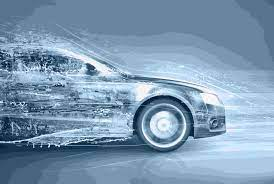
\includegraphics[width=0.7\columnwidth]{Figure}
	\caption{Add the caption to each figure! The caption should completely describe the figure so that the reader should be able to understand it without the need of reading the main text.}
	\label{fig:FigureA}
\end{figure}
Use the environment \textit{ref} to add a hyperlink to the figure. As example Figure \ref{fig:FigureA}.

\chapter{Application}

\section{Simulator description}
\begin{center}
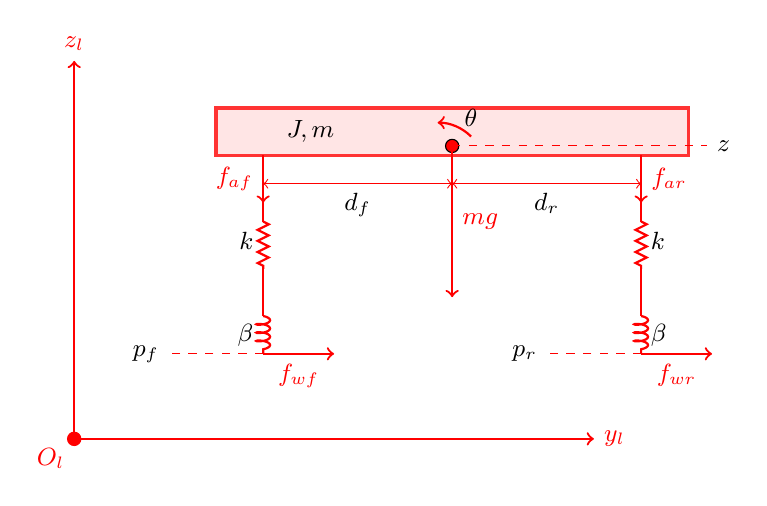
\begin{tikzpicture}[scale=1.2, every node/.style={font=\small}]
	
	% Coordinate axes
	\draw[->, thick, red] (-3.5,-1.5) -- (-3.5,2.5) node[above] {$z_l$};
	\draw[->, thick, red] (-3.5,-1.5) -- (2,-1.5) node[right] {$y_l$};
	\filldraw[red] (-3.5,-1.5) circle (2pt) node[below left] {$O_l$};
	
	% Sprung mass (body)
	\filldraw[color=red!80, fill=red!10, very thick] (-2,1.5) rectangle (3,2);
	\node at (-1,1.75) {$J, m$};
	
	% Center of mass
	\draw[fill=red] (0.5,1.6) circle (0.07);
	\draw[->, thick, red] (0.5,1.6) -- (0.5,0) node[midway,right] {$mg$};
	
	% pitch angle psi
	\draw[->, red, thick] (0,1.5) ++(0.7,0.2) arc[start angle=45,end angle=90,radius=0.5];
	\node at (0.7,1.9) {$\theta$};
	
	% Front suspension
	\draw[thick, red] (-1.5,1.5) -- (-1.5,0.8);
	\draw[thick, red, decorate, decoration={zigzag,segment length=4,amplitude=2}] (-1.5,0.8) -- (-1.5,0.3);
	\draw[thick, red] (-1.5,0.3) -- (-1.5,-0.2);
	\node[left] at (-1.5,0.6) {$k$};
	\draw[thick, red, decorate, decoration={coil,aspect=0.3, segment length=3}] (-1.5,-0.2) -- (-1.5,-0.6);
	\node[left] at (-1.5,-0.4) {$\beta$};
	\draw[->, thick, red] (-1.5,1.5) -- (-1.5,1.0) node[midway,left] {$f_{af}$};
	
	% Rear suspension
	\draw[thick, red] (2.5,1.5) -- (2.5,0.8);
	\draw[thick, red, decorate, decoration={zigzag,segment length=4,amplitude=2}] (2.5,0.8) -- (2.5,0.3);
	\draw[thick, red] (2.5,0.3) -- (2.5,-0.2);
	\node[right] at (2.5,0.6) {$k$};
	\draw[thick, red, decorate, decoration={coil,aspect=0.3, segment length=3}] (2.5,-0.2) -- (2.5,-0.6);
	\node[right] at (2.5,-0.4) {$\beta$};
	\draw[->, thick, red] (2.5,1.5) -- (2.5,1.0) node[midway,right] {$f_{ar}$};
	
	% Front and rear wheel forces
	\draw[->, thick, red] (-1.5,-0.6) -- (-0.75,-0.6) node[midway,below] {$f_{wf}$};
	\draw[->, thick, red] (2.5,-0.6) -- (3.25,-0.6) node[midway,below] {$f_{wr}$};
	
	% Ground heights
	\draw[dashed, red] (-1.5,-0.6) -- (-2.5,-0.6);
	\node[left] at (-2.5,-0.6) {$p_f$};
	\draw[dashed, red] (2.5,-0.6) -- (1.5,-0.6);
	\node[left] at (1.5,-0.6) {$p_r$};
	
	% Distances df and dr
	\draw[<->, red] (0.5,1.2) -- (-1.5,1.2);
	\node[below] at (-0.5,1.2) {$d_f$};
	\draw[<->, red] (0.5,1.2) -- (2.5,1.2);
	\node[below] at (1.5,1.2) {$d_r$};
	
	% Labels z
	\draw[dashed, red] (0.5,1.6) -- (3.2,1.6);
	\node[right] at (3.2,1.6) {$z$};
	
\end{tikzpicture}
\end{center}
Copy and past the Simulink block scheme and describe what each block does. Describe the set-up MATLAB file, where and how to change the parameters of the simulations. Remember to include also the sensor noises and realistic external disturbances.

\section{Simulation results}
Describe the simulation scenario: initial conditions, purpose of the simulation. Describe the results: are the results coherent with the expectation? If not why? Investigate the tuning: how the performance are affected by the selection of the parameters at disposal of the designer?

\chapter{Conclusions and further investigation}
Recap the main results obtained in the project and highlight eventual further investigation directions alogn which the performance could be improved. 

\newpage
\chapter*{Bibliography}
List the papers/books cited.

\newpage
\appendix
\chapter*{Appendix}
Use appendices to add technical parts which are instrumental for the completeness of the manuscript but are too heavy to be included inside the main text. Basically, appendices are exploited to let the main text cleaner and smoother. As example, the complete MATLAB listings can be reported in appendix.\\

HO

\end{document}          


\chapter{MAIN BODY}


\chapter{Application}

\chapter{Conclusions and further investigation}
 

\newpage
\chapter*{Bibliography}
List the papers/books cited.

\newpage
\appendix
\chapter*{Appendix}
Use appendices to add technical parts which are instrumental for the completeness of the manuscript but are too heavy to be included inside the main text. Basically, appendices are exploited to let the main text cleaner and smoother. As example, the complete MATLAB listings can be reported in appendix.\\


\end{document}          
